\section{Distributions}

In this section, various distribution functions are generated, which are used for generating data in mathematical simulations. 

\subsection{Uniform distribution}
In Uniform distribution, the random samples are generated with equal density as shown in Fig. \ref{fig:uniform_distribution}. The data for the figure is generated using Listing \ref{c:uniform_distribution} and saved in the file `uniform\_data.txt'; then data in the file is plotted using Python as show in Listing \ref{py:plot_uniform_dist}. 

\lstinputlisting[
language = C,
caption    = {Uniform distribution},
label      = {c:uniform_distribution}
]{distributions/uniform_distribution.c}

\lstinputlisting[
language = Python,
caption    = {Plot data generated by Listing \ref{c:uniform_distribution}},
label      = {py:plot_uniform_dist}
]{distributions/plot_uniform_dist.py}

\begin{figure}[!h]
	\centering
	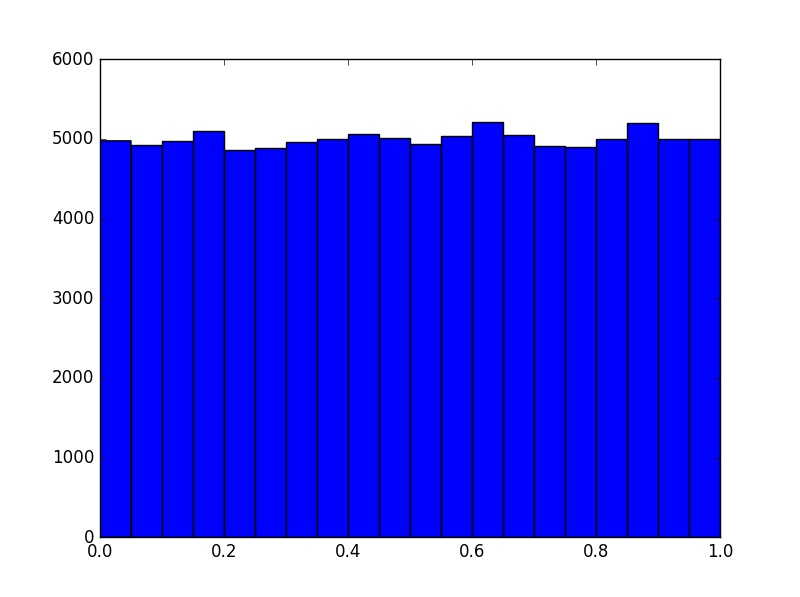
\includegraphics[scale = 0.5]{distributions/uniform_distribution}
	\caption{Uniform distributions generated by Listing \ref{c:uniform_distribution}}
	\label{fig:uniform_distribution}
\end{figure}


\subsection{Gaussian distribution}
Gaussian distribution can be implemented using `Box-Muller method'. This method uses `uniform distribution' for generating the Gaussian distribution, as shown at Lines 35-42 of Listing \ref{c:gaussian_distribution}. The results of the listing is plotted using Listing \ref{py:plot_gaussian_dist} and result is shown in Fig. \ref{fig:gaussian_distribution}.
\begin{figure}[!h]
	\centering
	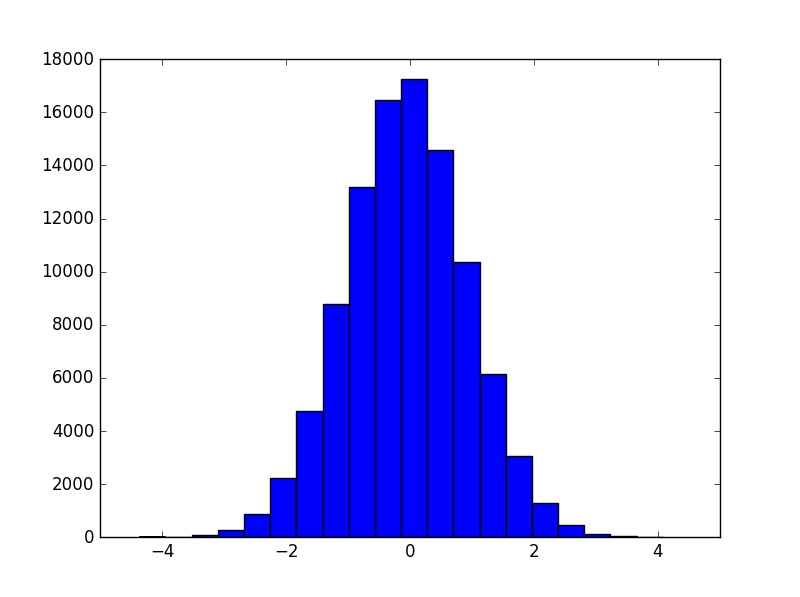
\includegraphics[scale = 0.5]{distributions/gaussian_distribution}
	\caption{Gaussian distributions generated by Listing \ref{c:gaussian_distribution}}
	\label{fig:gaussian_distribution}
\end{figure}

\lstinputlisting[
language = C,
caption    = {Gaussian distribution},
label      = {c:gaussian_distribution}
]{distributions/gaussian_distribution.c}

\lstinputlisting[
language = Python,
caption    = {Plot data generated by Listing \ref{c:gaussian_distribution}},
label      = {py:plot_gaussian_dist}
]{distributions/plot_gaussian_dist.py}

